%%%%%%%%%%%%%%%%%%%%%%%%%%%%%%%%%%%%%%%
% Wenneker Resume/CV
% LaTeX Template
% Version 1.1 (19/6/2016)
%
% This template has been downloaded from:
% http://www.LaTeXTemplates.com
%
% Original author:
% Frits Wenneker (http://www.howtotex.com) with extensive modifications by 
% Vel (vel@LaTeXTemplates.com)
%
% License:
% CC BY-NC-SA 3.0 (http://creativecommons.org/licenses/by-nc-sa/3.0/
%
%%%%%%%%%%%%%%%%%%%%%%%%%%%%%%%%%%%%%%

%----------------------------------------------------------------------------------------
%	PACKAGES AND OTHER DOCUMENT CONFIGURATIONS
%----------------------------------------------------------------------------------------

\documentclass[a4paper,12pt]{memoir} % Font and paper size

%%%%%%%%%%%%%%%%%%%%%%%%%%%%%%%%%%%%%%%%%
% Wenneker Resume/CV
% Structure Specification File
% Version 1.1 (19/6/2016)
%
% This file has been downloaded from:
% http://www.LaTeXTemplates.com
%
% Original author:
% Frits Wenneker (http://www.howtotex.com) with extensive modifications by 
% Vel (vel@latextemplates.com)
%
% License:
% CC BY-NC-SA 3.0 (http://creativecommons.org/licenses/by-nc-sa/3.0/)
%
%%%%%%%%%%%%%%%%%%%%%%%%%%%%%%%%%%%%%%%%%

%----------------------------------------------------------------------------------------
%	PACKAGES AND OTHER DOCUMENT CONFIGURATIONS
%----------------------------------------------------------------------------------------

\usepackage{XCharter} % Use the Bitstream Charter font
\usepackage[utf8]{inputenc} % Required for inputting international characters
\usepackage[T1]{fontenc} % Output font encoding for international characters

\usepackage[top=1cm,left=0cm,right=1cm,bottom=1cm]{geometry} % Modify margins

\usepackage{graphicx} % Required for figures

\usepackage{flowfram} % Required for the multi-column layout

\usepackage[hidelinks]{hyperref} % URLs

\usepackage[usenames,dvipsnames]{xcolor} % Required for custom colours

\usepackage{tikz} % Required for the horizontal rule

\usepackage{enumitem} % Required for modifying lists
\setlist{noitemsep,nolistsep} % Remove spacing within and around lists

\setlength{\columnsep}{\baselineskip} % Set the spacing between columns

% Define the left frame (sidebar)
\newflowframe{0.2\textwidth}{\textheight}{0pt}{0pt}[left]
\newlength{\LeftMainSep}
\setlength{\LeftMainSep}{0.2\textwidth}
\addtolength{\LeftMainSep}{1\columnsep}
 
% Small static frame for the vertical line
\newstaticframe{1.5pt}{\textheight}{\LeftMainSep}{0pt}
 
% Content of the static frame with the vertical line
\begin{staticcontents}{1}
\hfill
\tikz{\draw[loosely dotted,color=RoyalBlue,line width=1.5pt,yshift=0](0,0) -- (0,\textheight);}
\hfill\mbox{}
\end{staticcontents}
 
% Define the right frame (main body)
\addtolength{\LeftMainSep}{1.5pt}
\addtolength{\LeftMainSep}{1\columnsep}
\newflowframe{0.7\textwidth}{\textheight}{\LeftMainSep}{0pt}[main01]

\pagestyle{empty} % Disable all page numbering

\setlength{\parindent}{0pt} % Stop paragraph indentation

%----------------------------------------------------------------------------------------
%	NEW COMMANDS
%----------------------------------------------------------------------------------------

\newcommand{\userinformation}[1]{\renewcommand{\userinformation}{#1}} % Define a new command for the CV user's information that goes into the left column

\newcommand{\cvheading}[1]{{\Huge\bfseries\color{RoyalBlue} #1} \par\vspace{.6\baselineskip}} % New command for the CV heading
\newcommand{\cvsubheading}[1]{{\Large\bfseries #1} \bigbreak} % New command for the CV subheading

\newcommand{\Sep}{\vspace{1em}} % New command for the spacing between headings
\newcommand{\SmallSep}{\vspace{0.5em}} % New command for the spacing within headings

\newcommand{\aboutme}[2]{ % New command for the about me section
\textbf{\color{RoyalBlue} #1}~~#2\par\Sep
}
	
\newcommand{\CVSection}[1]{ % New command for the headings within sections
{\Large\textbf{#1}}\par
\SmallSep % Used for spacing
}

\newcommand{\CVSectionNoSep}[1]{ % New command for the headings within sections
{\Large\textbf{#1}}\par
% \SmallSep % Used for spacing
}

\newcommand{\CVItem}[2]{ % New command for the item descriptions
\textbf{\color{RoyalBlue} #1}\par
#2
\SmallSep % Used for spacing
}

\newcommand{\CVItemNoSep}[2]{ % New command for the item descriptions
\textbf{\color{RoyalBlue} #1}\par
#2
% \SmallSep % Used for spacing
}

\newcommand{\bluebullet}{\textcolor{RoyalBlue}{$\circ$}~~} % New command for the blue bullets
 % Include the file specifying document layout and packages

%----------------------------------------------------------------------------------------
%	NAME AND CONTACT INFORMATION 
%----------------------------------------------------------------------------------------

\userinformation{ % Set the content that goes into the sidebar of each page
\begin{flushright}
% Comment out this figure block if you don't want a photo
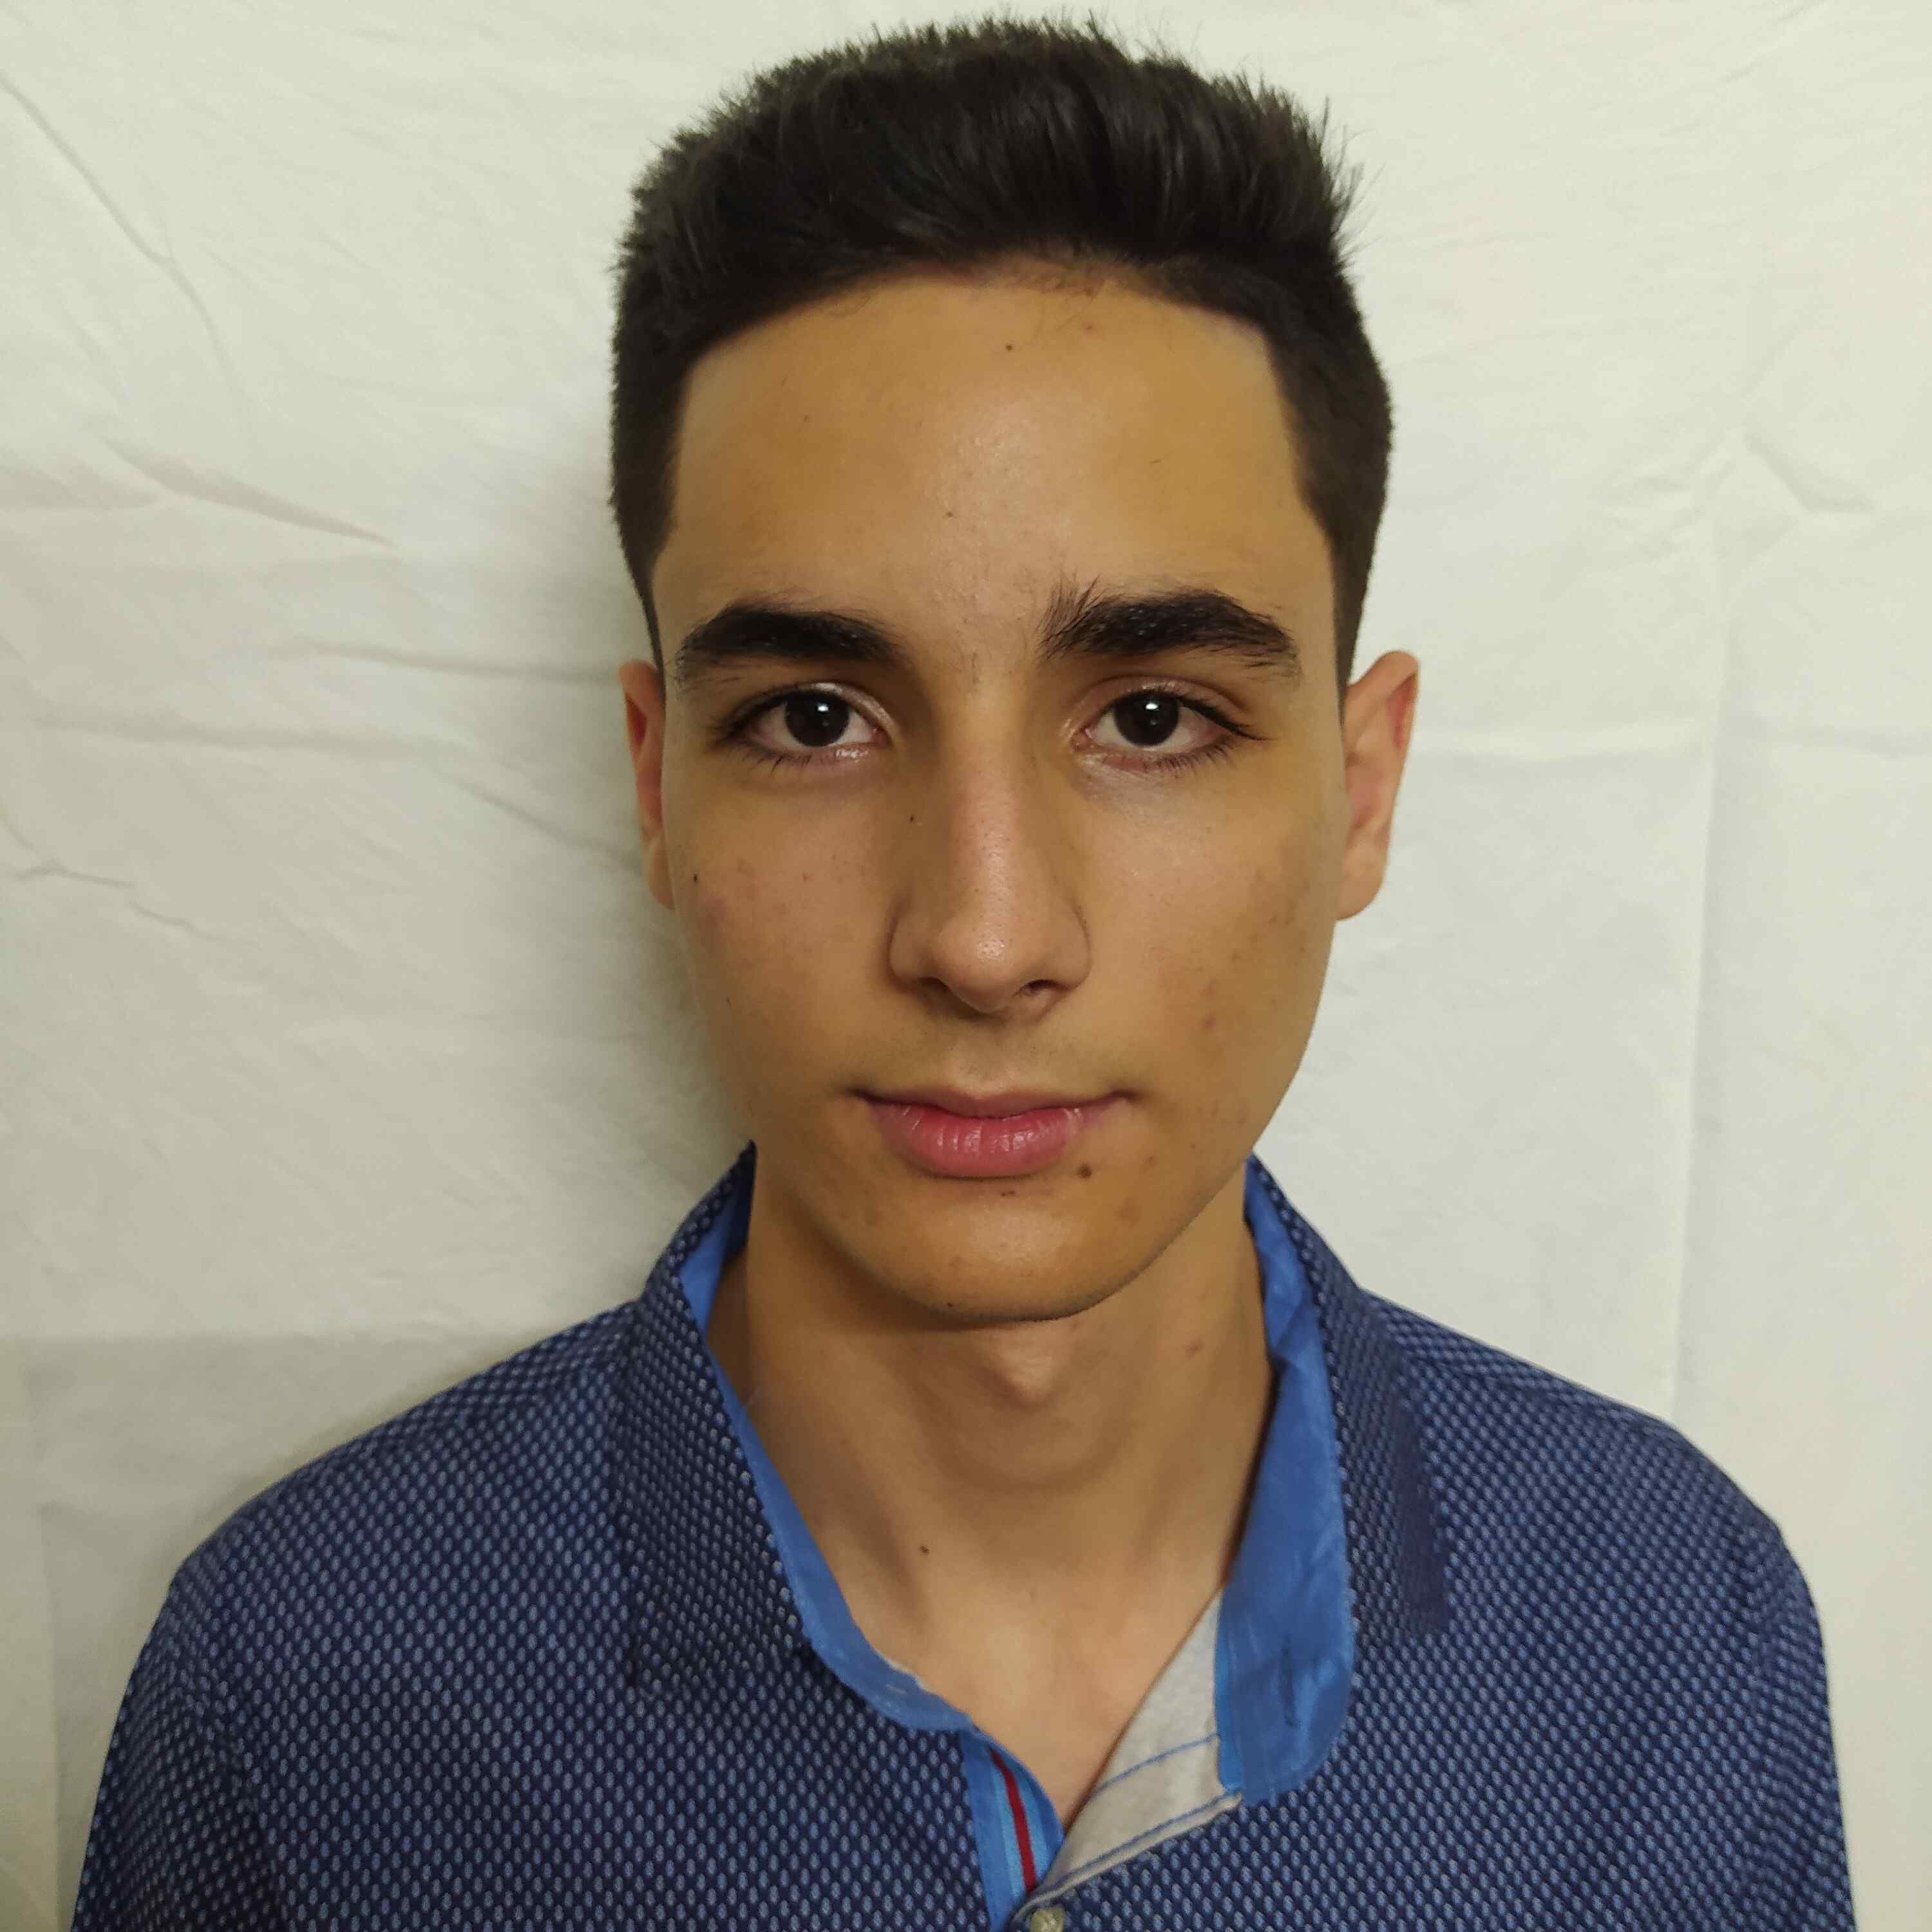
\includegraphics[width=0.6\columnwidth]{photo.jpg}\\[\baselineskip] % Your photo
\small % Smaller font size
Humberto Yusta Gómez \\ % Your name
\Sep % Some whitespace
\href{mailto://humbertoyusta02@gmail.com}{humbertoyusta02@ gmail.com} \\ % Your email address
\Sep % Some whitespace
% \url{www.johnsmith.com} \\ % Your URL
+53 55743975  \\ % Your phone number
\Sep % Some whitespace
\textbf{Dirección} \\
Calle Maceo \#20 \\ % Address 1
Zulueta, Remedios \\ % Address 2
Villa Clara, Cuba \\ % Address 3
\Sep % Some whitespace
GitHub \\
\href{https://github.com/humbertoyusta}{humbertoyusta} \\
\Sep % Some whitespace
LinkedIn \\
\href{https://linkedin.com/in/humberto-yusta-036710212}{humberto-yusta-036710212}
\vfill % Whitespace under this block to push it up under the photo
\end{flushright}
}

%----------------------------------------------------------------------------------------

\begin{document}

\userinformation % Print your information in the left column

\framebreak % End of the first column

%----------------------------------------------------------------------------------------
%	HEADING
%----------------------------------------------------------------------------------------

\cvheading{Humberto Yusta Gómez} % Large heading - your name

\cvsubheading{Estudiante, Programador Competitivo} % Subheading - your occupation/specialization

%----------------------------------------------------------------------------------------
%	ABOUT ME
%----------------------------------------------------------------------------------------

\aboutme{Acerca de mí}{Graduado de preuniversitario con cinco años de experiencia en programación competitiva. 
Apasionado de las matemáticas y las ciencias de la computación, Dedicado al aprendizaje continuo, al desarrollo profesional, 
y dispuesto a aprender nuevas tecnologías y herramientas si surge la necesidad.}

%----------------------------------------------------------------------------------------
%	EXPERIENCE
%----------------------------------------------------------------------------------------

\CVSection{Experiencia}

%------------------------------------------------

\CVItem{2018 - Presente, \textit{Programador Competitivo}}{
Resultados destacados:
\begin{itemize}
	\item \href{https://stats.ioinformatics.org/people/7078}{Medalla de Bronce} en la Olimpiada Internacional de Informática (\href{https://ioi2020.sg}{IOI 2020}), obteniendo el mejor resultado de Latinoamérica.
	\item \href{https://codeforces.com/profile/humbertoyusta}{Maestro} en codeforces.com, \href{https://atcoder.jp/users/humbertoyusta}{División amarillo} en atcoder.jp, División Platino en usaco.org
	\item Medalla de Oro (3er lugar), Medalla de Bronce, y Medalla de Plata en la Competencia Iberoamericana de Informática y Computación(CIIC) 2020, 2019 y 2018 respectivamente.
	\item 3er lugar en la Ronda de Clasificación a la Final Caribeña de ICPC 2020, 6to lugar en la Final Caribeña de ICPC 2019. Participando como invitado en ambas.
	\item Medalla de Oro en la Olimpiada Cubana de Informática, en 2020, 2019 y 2018. Lugares 1ro, 2do y 13 respectivamente.
	\item Octavo lugar en el Concurso Abierto de la Olimpiada de Informática de Asia-Pacífico (APIO 2020).
\end{itemize}
}

%------------------------------------------------

\CVItem{2021 - Presente, \textit{Entrenador y Autor de Problemas}}{Trabajo Voluntario
\begin{itemize}
	\item Autor de problemas y organizador de las siguientes competencias de programación:
		\begin{itemize}
			\item \href{https://codeforces.com/blog/entry/99299}{Ronda de Codeforces \#768 (Div. 1, Div. 2)}, la cual tuvo más de 26000 participantes.
			\item Competencia Iberoamericana de Informática y Computación 2022
			\item Competencia Iberoamericana de Informática y Computación 2021
			\item Olimpiada Cubana de Informática 2022
			\item Competencia de Selección del Equipo de Cuba para las Olimpiadas Internacionales 2021
		\end{itemize}
	\item Autor de 3 artículos educativos en codeforces.
	\item Entrenador del equipo de Cuba para la IOI 2021 durante dos semanas.
\end{itemize}
}

%------------------------------------------------

\Sep % Extra whitespace after the end of a major section

%----------------------------------------------------------------------------------------
%	EDUCATION
%----------------------------------------------------------------------------------------

\CVSection{Educación}

%------------------------------------------------

\CVItem{Sep. 2017 - Ago. 2020, IPVCE Ernesto Che Guevara}{Graduado de preuniversitario \\
Reconocido como uno de los mejores graduados del Centro de Entrenamiento para Concursos de Conocimiento.}

%------------------------------------------------

\Sep % Extra whitespace after the end of a major section

%----------------------------------------------------------------------------------------
%	COMMUNICATION SKILLS
%----------------------------------------------------------------------------------------

% \CVSection{Communication Skills}

%------------------------------------------------

% \CVItem{2015, \textit{Oral Presentation}, California Business Conference}{Presented research I conducted for my Masters of Engineering degree.}

%------------------------------------------------

% \CVItem{2014, \textit{Poster}, Annual Business Conference (Oregon)}{As part of the course work for BUS320, I created a poster analyzing several local businesses and presented this at a conference.}

%------------------------------------------------

% \Sep % Extra whitespace after the end of a major section

%----------------------------------------------------------------------------------------
%	SKILLS
%----------------------------------------------------------------------------------------

\CVSectionNoSep{Habilidades de programación}

%------------------------------------------------

\CVItemNoSep{Lenguajes de programación}
{\begin{tabular}{p{0.2\textwidth} p{0.2\textwidth} p{0.2\textwidth} p{0.2\textwidth}}
\bluebullet C++ &  \bluebullet Java & \bluebullet Typescript & \bluebullet Python\\
\end{tabular}}

%------------------------------------------------

\CVItemNoSep{Software de Desarrollador}
{\begin{tabular}{p{0.2\textwidth} p{0.2\textwidth} p{0.2\textwidth} p{0.2\textwidth}}
\bluebullet Git &  \bluebullet NestJS & \bluebullet PostgreSQL & \bluebullet Polygon\\
\end{tabular}}

%------------------------------------------------

% \CVItemNoSep{Programming Skills}
% {\begin{tabular}{p{0.2\textwidth} p{0.2\textwidth}}
%  \bluebullet Data Structures and Algorithms &  \bluebullet Mathematical Skills\\
% \end{tabular}}

%------------------------------------------------

% \Sep % Extra whitespace after the end of a major section

%----------------------------------------------------------------------------------------
%	NEW PAGE DELIMITER
%	Place this block wherever you would like the content of your CV to go onto the next page
%----------------------------------------------------------------------------------------

% \clearpage % Start a new page

% \userinformation % Print your information in the left column

% \framebreak % End of the first column

%----------------------------------------------------------------------------------------
%	AWARDS
%----------------------------------------------------------------------------------------

% \CVSection{Awards}

%------------------------------------------------

% \CVItem{2010, \textit{Postgraduate Scholarship}, Cornell University}{Awarded to the top student in their final year of a Bachelors degree.}

%------------------------------------------------

% \Sep % Extra whitespace after the end of a major section

%----------------------------------------------------------------------------------------
%	INTERESTS
%----------------------------------------------------------------------------------------

% \CVSection{Interests}

%------------------------------------------------

% \CVItem{Professional}{Data analysis, company profiling, risk analysis, economics, web design, web app creation, software design, marketing}

%------------------------------------------------

% \CVItem{Personal}{Piano, chess, cooking, dancing, running}

%------------------------------------------------

% \Sep % Extra whitespace after the end of a major section

%----------------------------------------------------------------------------------------

\end{document}
